\chapter{Introducción}
El crear modelos para la visualización de datos ayuda a observar con mayor claridad los datos para encontrar relaciones entre ellos.

El \emph{aprendizaje máquina}\footnote{Traducido como machine learning en inglés, tiene como objetivo desarrollar técnicas que les permitan a las computadoras aprender.} es un área dentro de la \emph{ciencia de datos}\footnote{Traducido como data science en inglés, involucra métodos para extraer conocimiento de datos, eso con la finalidad de que haya un mejor entendimiento de los datos.} que puede ayudar a crear dichos modelos para tener una más eficiente visualización cuando se trabaja con una gran cantidad de datos, que es lo que se requiere para el presente trabajo. El área de la ciencia de datos es muy útil ya que permite trabajar con grandes cantidades de datos aminorando la cantidad de tiempo empleado en la creación de gráficos que permitan visualizar los datos.

La tarea en el presente proyecto es utilizar modelos para visualizar las relaciones entre los contaminantes del aire y salud pública, para ello se requieren datos sobre salud pública y sobre los niveles de contaminantes del aire.

Para la realización de los experimentos se tienen datos de ingresos hospitalarios provenientes de la base de datos de la Secretaría de Salud del Gobierno de México. También se tienen registros de los niveles de algunos contaminantes del aire presentes en el área metropolitana de Monterrey, dichos registros son hechos por las estaciones mostradas en la figura \ref{estaciones}.

\begin{figure}[h!]
\setcounter{figure}{0} % por culpa de sciposter
\captionsetup{type=figure} % por culpa de sciposter
\begin{center}
   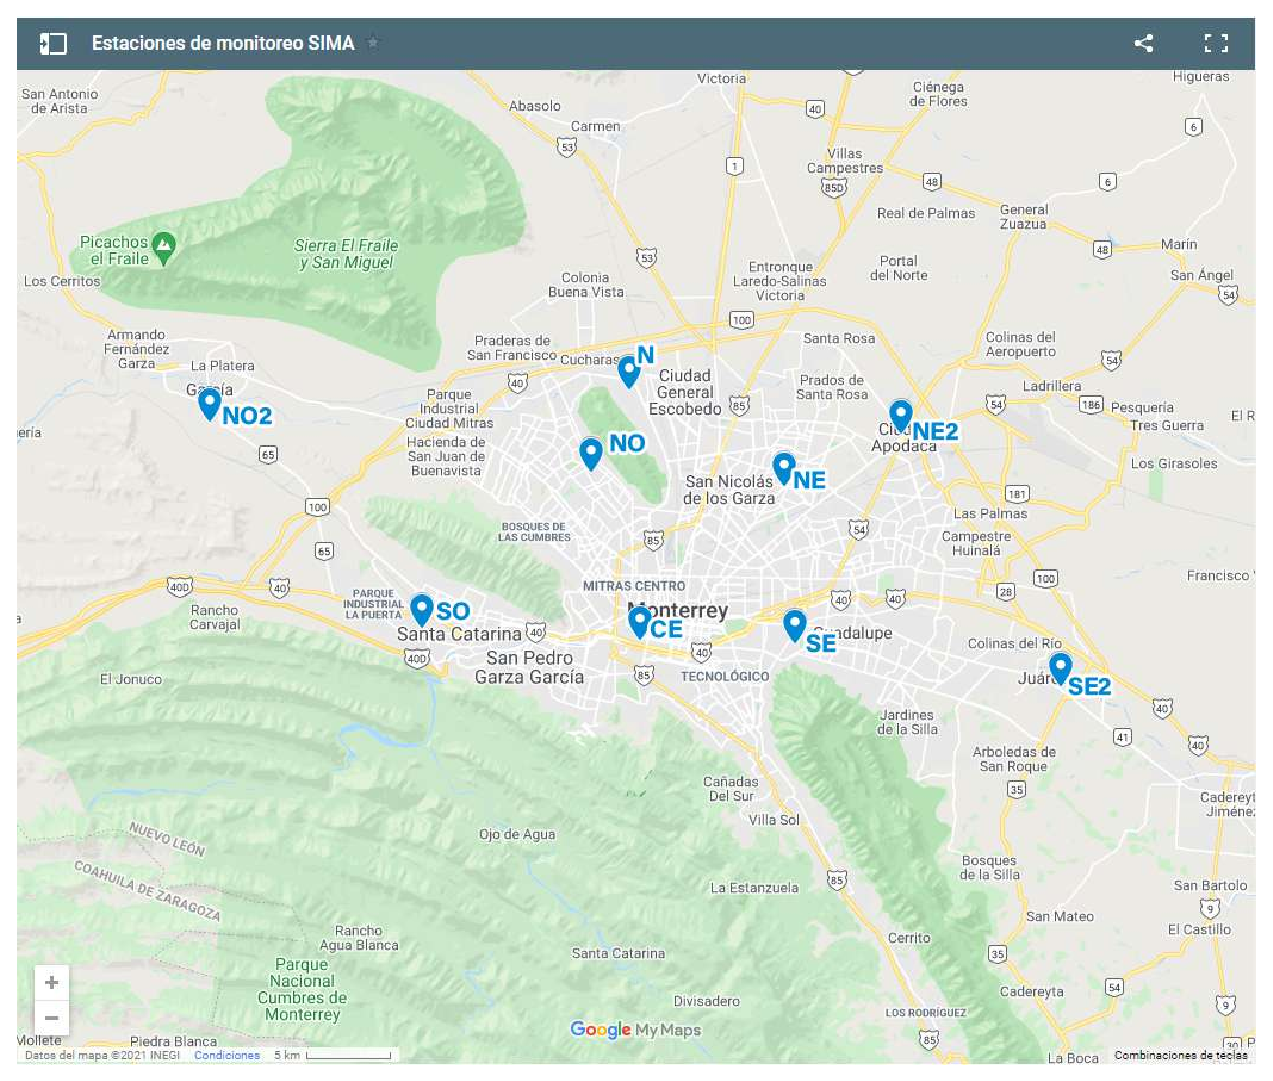
\includegraphics[width=1\textwidth]{mapa_estaciones.eps}
   \end{center}
    \caption{Localización de las estaciones de monitoreo de la calidad del aire.}
    \label{estaciones}
\end{figure}

\clearpage

\section{Motivación}
Existen investigaciones que ya han estudiado las relaciones entre contaminantes del aire y salud pública, sin embargo, con el presente trabajo se busca aportar a la creación de nuevas herramientas que permitan observar y estudiar dichas relaciones. El poder visualizar dichas relaciones puede ayudar a tomar medidas adecuadas que permitan aminorar los efectos negativos de los contaminantes del aire en la salud de las personas.

\section{Hipótesis}
Se plantea que con modelos de regresión se pueden obtener gráficos donde se pueden observar las relaciones entre el número de ingresos hospitalarios y los niveles de contaminantes del aire.

\section{Objetivos}
En esta sección se establece el objetivo general y los objetivos específicos sobre los que se orienta la tesis.

\subsection{Objetivo general}
El objetivo de generar un módelo que muestra las relaciones existentes entre contaminantes del aire y salud pública tiene la finalidad de apoyar a la implementación de estrategías que aminoran los efectos negativos de los contaminantes del aire en la salud de las personas. Con el modelo generado se puede tener una herramienta que permite visualizar graficamente las relaciones con solo proporcionarle el conjunto de datos.

\subsection{Objetivos específicos}
\begin{itemize}
\item Generar un módelo de regresión que permite visualizar las relaciones entre contaminantes del aire y salud pública a partir de un conjunto de datos.
\end{itemize}
\begin{itemize}
\item Generar un módelo de regresión que muestra un análisis de datos proporcionados sobre niveles de contaminantes del aire y salud pública.
\end{itemize}
\begin{itemize}
\item Generar un módelo de regresión que permite estudiar las relaciones entre los niveles de contaminantes del aire y salud pública.
\end{itemize}

%\section{Estructura}
%El contenido de la investigación se divide en...


\chapter{Antecedentes}
%En algunos trabajos se han utilizado modelos de series de tiempo y ...

\section{Antecedentes históricos}
\citet{r1} menciona que uno de los diseños epidemiológicos más utilizados son los estudios de series temporales. Con esos diseños se analizan las variaciones en el tiempo de la exposición al contaminante y el indicador de salud estudiado en una población.

\section{Salud en una comunidad}
Existen factores ambientales que afectan la salud de una comunidad como: el abastecimiento de agua potable y el saneamiento, la vivienda y el hábitat, la alimentación, la contaminación ambiental, el empleo de productos químicos y los riesgos ocupacionales \citep{r2}.

\chapter{Estado del arte}
En este capítulo se explica...

\section{Investigaciones relacionadas}
Existen algunos trabajos que...

\section{Comparación de trabajos}
La mayoría de los trabajos citados...

\subsection{Comparaciones}
En el cuadro...

\subsection{Áreas de oportunidad}
En el cuadro...


\chapter{Solución propuesta}
Habiendo conocido las características que mejor describen a los atributos del presente trabajo, se puede decir que la base del método propuesto se puede desarrollar...

\section{Datos recolectados}
Inicialmente...


\chapter{Desarrollo de la solución}
Recapitulando las fases anteriores, se conoce que...


\chapter{Experimentos}
Después de...

\section{Diseño experimental}
Hola...

\section{Resultados}
Establecidos los experimentos que se van a realizar, se reporta los resultados obtenidos...

\section{Discusión}
Todos los experimentos son ejecutados en una laptop con las especificaciones del cuadro \ref{tab:Especificaciones técnicas del PC}.

\begin{table}[H]
	{\centering
		\caption{Especificaciones técnicas del equipo de cómputo}
		\begin{tabular}{|c|c|c|}
			\hline
			Sistema Operativo & Windows 10 64 bits\\
			\hline
			Procesador & Intel Core i5-7300HQ\\
			\hline
			RAM & 8 GB RAM DDR4 2133 MHz\\
			\hline
		\end{tabular}

	\label{tab:Especificaciones técnicas del PC}
	}
\end{table}


\chapter{Conclusiones}
Este capítulo describe la tesis a partir de la manera que cumple los objetivos generales y específicos para determinar si la hipótesis se comprueba, trata también del porque se realizó la tesis...

\clearpage

\section{Contribuciones}
La solución propuesta surgió a partir de...

\section{Trabajo a futuro}
La solución propuesta en la tesis...